\def\length{sqrt(1+(x-y)^2)}
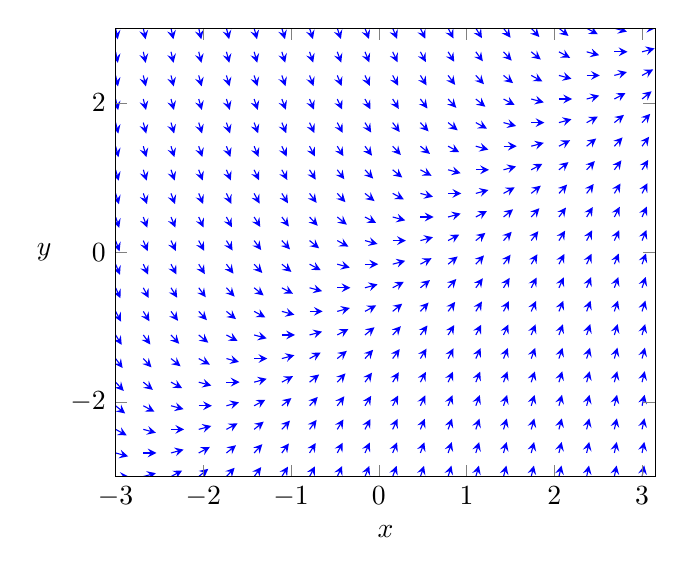
\begin{tikzpicture}
\begin{axis}[domain=-3:3, view={0}{90},xlabel = $x$,ylabel=$y$,ylabel style={rotate=-90},]
\addplot3[blue, quiver={u={1/(\length)}, v={(x-y)/(\length)}, scale arrows=0.15}, -stealth,samples=20] {0};
\end{axis}
\end{tikzpicture}
